\documentclass{article}
\usepackage[utf8]{inputenc}

\usepackage{fullpage}

\usepackage{tikz}
%\usetikzlibrary{calc,arrows,shapes,backgrounds,patterns,fit,decorations,decorations.pathmorphing}

\usepackage[shadow,colorinlistoftodos,textwidth=2.5cm]{todonotes}
\usepackage[final,colorlinks,hyperindex,unicode=true,pdftitle=SPAdes Manual,]{hyperref}
\usepackage{url}

\def\spades{SPAdes}

\usepackage{listings}
\definecolor{light-gray}{gray}{0.92}
\lstset{basicstyle=\ttfamily,framerule=0pt,frame=single,backgroundcolor=\color{light-gray}}

%\newenvironment{mycode}
%  {\begin{lstlisting}}
%  {\end{lstlisting}}

\begin{document}
\title{{\spades} Manual\\{\small Revision: \today}}
\date{}
\maketitle

%\begin{abstract}
{\spades} stands for St.~Petersburg genome assembler.
It is intended for both single cell and standard (multicell) 
assemblies. This manual will help you to install and run
{\spades}.\todo{Valera, is it possible to give some quick start guide for impatient users here? Smth like {\tt install}-{\tt make}-{\tt run}.}


%\end{abstract}

\renewcommand{\contentsname}{}
\tableofcontents

\pagebreak

\listoftodos

\pagebreak

\section{How to read the manual}
\subsection{Notation}
Throughout all the document we assume that mate reads are oriented 
towards each other. Read size, distance, gap, and insert length are 
explained in the picture below.\todo{Valera, anything else to be explained here?}

\begin{center}
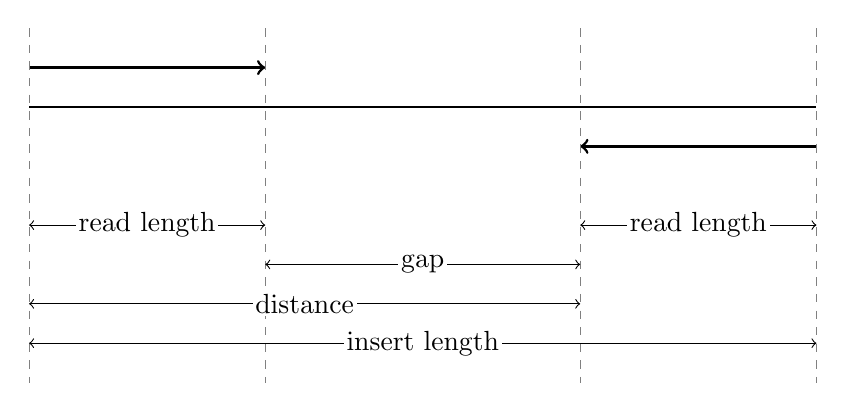
\begin{tikzpicture}
%\draw[help lines] (0,-3) grid (10,3);
\draw[line width=1pt] (0,2) -- (10,2);
\draw[line width=1pt,->] (0,2.5) -- (3,2.5);
\draw[line width=1pt,->] (10,1.5) -- (7,1.5);

\foreach \x in {0, 3, 7, 10}
  \draw[dashed,gray] (\x,3) -- (\x,-1.5);

\foreach \f/\s/\y/\t in {0/3/0.5/read length, 7/10/0.5/read length, 3/7/0/gap, 0/7/-0.5/distance, 0/10/-1/insert length}
\path[<->,draw] (\f,\y) -- node[fill=white,inner sep=1pt,rectangle] {\t} (\s,\y);

\end{tikzpicture}
\end{center}

\subsection{Config files and commands}
Config files and commands are given in gray boxes. 
Note that the text can be copy-pasted directly from this document.
%Note also that all the links and all the colored text in the manual are clickable.

In config files, parts of lines starting with a semicolon are just cooments.


\section{Requirements}\label{section:requirements}
\subsection{Packages}
The following packages are required for using {\spades}.
For each of the packages, you can either install it by 
the given command or download it from the given webpage.{\todo{Valera, do we need these webpages here?}}
\todo{Valera, is it possible to install everything by pressing just one button?}

\begin{itemize}
  \item {\tt gcc} version 4.4 or later
  \begin{lstlisting}
  sudo apt-get install gcc
  \end{lstlisting}
  \url{http://gcc.gnu.org}

  \item {\tt cmake} version 2.6 or later
  \begin{lstlisting}
  sudo apt-get install cmake
  \end{lstlisting}

  \item {\tt log4cxx}
  \begin{lstlisting}
  sudo apt-get install liblog4cxx10-dev
  \end{lstlisting}

  \item {\tt boost} version 1.42 (exactly this version!)
  \begin{lstlisting}
  sudo apt-get install libboost-all-dev
  \end{lstlisting}

  \item {\tt zlib}
  \begin{lstlisting}
  sudo apt-get install zlib-bin
  \end{lstlisting}
\end{itemize}

\subsection{RAM}
\todo{Valera, add RAM requirements/suggestions}


\section{Getting {\spades}}
\subsection{Webpage}
The latest version of the source code can be downloaded from\\
\url{http://bioinf.spbau.ru/spades}\todo{Valera, are we going to put pre-compiled binaries also?}

To extract the contents of the downloaded archived file run:
\begin{lstlisting}
tar -xzf <dir> spades.tar.gz
\end{lstlisting}
where {\tt <dir>} is the destination directory.

\subsection{Git repository}
Alternatively, you can pull the source code from the 
repository:\todo{Valera, are we going to provide such an option?}
\begin{lstlisting}
git clone ...
\end{lstlisting}


\section{Compiling}
When all the required packages are installed (see 
Section~\ref{section:requirements})
just run
\begin{lstlisting}
make <K>
\end{lstlisting}
in the root directory. Here {\tt <K>} is the $k$-mer size.
The default value is $55$ (and it is recommended for reads of length $100$).

\section{Preparing input data}
\subsection{Correcting errors in your dataset}
\todo{Sergey Nikolenko?..}

\subsection{Adding your dataset to the config file}
{\spades} requires paired reads to be in separate files.
Additionally, {\spades} can use unpaired reads that normally appear after discarding one read of the paired read in error correction step.
Thus input reads should be arranged into four files: paired reads left parts, paired reads right parts, unpaired reads which originally were left parts, and
unpaired reads which originally were right parts. Thus, the first two files should contain the same number of reads, while
there are no requirements on the number of reads in the last two files (any of them can even be empty).
Files are expected to be in fasta or fastq formats and can be compressed.

In file {\tt src/debruijn/datasets.info} add a new entry according to the following self-explaining pattern (recall that parts of lines starting from
semicolon are comments):
\begin{lstlisting}
ECOLI_IS220_QUAKE
{
  first            E.coli/is220/s_6_1.cor.fastq.gz ; paired left
  second           E.coli/is220/s_6_2.cor.fastq.gz ; paired right
  single_first     E.coli/is220/s_6_1.cor_single.fastq.gz ; unpaired left
  single_second    E.coli/is220/s_6_2.cor_single.fastq.gz ; unpaired right
  RL               100 ; read length
  IS               220 ; insert size
  single_cell      false ; true if input data was obtained 
                         ; with mda (single cell) technology
  reference_genome E.coli/MG1655-K12.fasta.gz ; optional
}
\end{lstlisting}

%This defines the dataset with the name {\tt ECOLI_IS220_QUAKE}. The first four lines give (relative) paths
%to four types of reads explained above. The paramater {\tt RL} defines an approximate read length.
%{\tt IS} defines approximate insert size.


%DATASET\_NAME
%\{
%\begin{itemize}
%\item {\it first} path rto file with left parts of paired reads
%\item{\it second} path to file with right parts of paired reads
%\item{\it single\_first} path to file with unpaired reads which originally were left parts
%\item{\it single\_second} path to file with unpaired reads which originally were right parts
%\item{\it jumping\_first} Separate section should be written about these three parameters. For now you can just skip this parameters and not to include them here.
%\item{\it jumping\_second}
%\item{\it jump\_is} 
%\item{\it RL} Approximate length of reads in the input.
%\item{\it IS} Approxmiate insert size of input paired reads
%\item{\it single\_cell} true if input data was obtained with mda (single cell) technology and false otherwise. Parameters to be used in graph simplification procedures depend on this parameter
%\item{\it reference\_genome} Path to file with reference genome if available otherwise just skip this parameter
%\item{\it LEN} Approximate total size of genome to be assembled
%\end{itemize}
%\}



\section{Preparing configuration files}
\todo[inline]{Valera, I've left this section as it is since you are going to change the structure of configs.}
Our configs are organized into four files: {\tt configs.info}, {\tt simplification.info}, {\tt distance\_estimation.info} and {\tt detail\_info\_printer.info}. 
All of them are located in directory {\tt src/debruijn}.

Note that semicolon sign in the config format that is used in our assembler marks all the remaining as comment and is ignored.
in order to fill these files with default values one should run
\begin{lstlisting}
./cpcfg
\end{lstlisting}
in the root directory.

\subsection{Main parameters}
\begin{itemize}
\item {\it dataset} the name of dataset as it was in datasets.info file (see ``Create dataset entry'' section)
\item {\it entry point} parameter defines the starting point of assembler run.
In case this parameter is set to the value other than ``construction'' assembler loads save files which were created on the previous assembler run and thus continues previous run from the corresponding point.
All possible values of this parameter can be found commented in default configs.
The most useful of them are:
\begin{itemize}
\item {\it construction} run assembler from the very beginning.
\item {\it simplification} run assembler from graph simplification step in case you would like to rerun assembler with different simplification parameters or draw some graph pictures (see ``Pictures'' section).
\item {\it repeats\_resolving} run assembler from repeats resolving step in case you would like to rerun assembler with different resolving parameters or even with another repeats resolving.
\end{itemize}
\item {\it use\_additional\_contigs} parameter indicates whether additioanl contigs should be used for graph constraction.

Normally these contigs are obtained from the previous iterations of iterative run of Spades thus 
in most cases this parameter should be \textbf{true for iterative run of Spades} 
and false otherwise (see ``Run Spades'' section for further details).

Later this parameter will be removed and its value will be automatically generated based on the type of run.
\item {\it paired\_mode} parameter indicates whether assembler should be run in single reads mode or in paired reads mode. 
In single reads mode paired info is not collected and thus repeat resolving step is not performed. Single mode is much faster and recommended
for the first assembly attempt (repeat resolving can be applied later)
\item {\it resolving\_mode} parameter defines which of our repeat resolving algorithms should be used.
Currently there are ``none'', ``dima'', ``andrey'', ``combined'' and ``jump'' modes. (As for now use ``dima'' mode by default).
These modes should be discribed in the release version of this manual. 

\textbf{Important.} Repeat resolution won't happen if paired\_mode is set to false.
\end{itemize}

A sample config file if given below.
\begin{lstlisting}
; input options:

#include "src/debruijn/simplification.info"
#include "src/debruijn/datasets.info"
#include "src/debruijn/distance_estimation.info"

dataset       QUAKE_CROPPED_400K
;dataset              LB_QUAKE_FULL

input_dir      ./data/input/
output_base      ./data/debruijn/

additional_contigstmp_contigs.fasta

load_from         latest/saves/ ; tmp or latest 

entry_point construction
;entry_point paired_info_count
;entry_point simplification
;entry_point late_pair_info_count
;entry_point distance_estimation
;entry_point repeats_resolving
;entry_point n50_enlargement

; iterative mode switcher, activates additional contigs usage
use_additional_contigs false

; use single reads if they are provided
use_single_reads true

; paired (1) or unpaired (0, for quick debug and algorithms testing) mode
paired_mode true

; set it true to get statistics, such as false positive/negative, perfect match, etc.
paired_info_statistics false

; use advanced distance estimation or not
advanced_estimator_mode true

; set to true to obtain paired info from genome mapping rather than from paired reads
etalon_info_mode  false

; Collect paired information before or after graph simplification
late_paired_info true

; Produce info for all components of graph and run repeat resolver for each component.
componential_resolve true
\end{lstlisting}

\subsection{Simplification parameters}

File is divided into two parts: for single cell and for multicell assembly depending on the value of ``single\_cell'' flag in dataset parameters (see section ``Create dataset entry'').

The most common parameter to vary here is ec::max\_coverage (parameter max\_coverage in ec section). It determines the coverage of edges that should be checked for being erroneous. Don't put large values here before some preliminary analysis of pictures was made. 15-20 should be more than enough for first attempt.


\subsection{Printing parameters}


\section{Running}
There are basically two ways to run {\spades}: normal and iterative. 
The difference is that the normal run uses a fixed value of $k$,
while the iterative run uses several values.

\subsection{Normal run}
Recall that the value of $k$ is given to {\spades} through the {\tt make} command:
\begin{lstlisting}
make <K>
\end{lstlisting}
After this, just run
\begin{lstlisting}
./run
\end{lstlisting}
It is a good idea to redirect the output stream to a file since there is a fair bit of logs that is printed to console.


\subsection{Iterative run}
This is recommended for datasets with low coverage or with unevenly distributed coverage.
%(but you can use it in all the cases if you have some time and patience to wait). 
In order to launch iterative run just run 
\begin{lstlisting}
./iterative_run <K_1> <K_2> ... <K_m>
\end{lstlisting}
where {\tt K\_i}'s is the sequence of values of $k$ to be used by iterative run.
Normally, we use the sequence 21 33 55 (there even is a separate script {\tt iterative\_run\_21\_33\_55}).
Preliminary compilation is not required for iterative run since this script compiles the code itself.

\textbf{Important!} Do not forget to set use\_additional\_contigs parameter = true and paired\_mode = false for iterative run!{\todo{Valera, is it possible to check these flags automatically?}}

During iterative run, logs are be written to console and to files in {\tt logs/DATE\_TIME/...}.
The symlink {\tt latest} in the folder {\tt logs} leads to the latest run logs' folder.

\section{Understanding the output}
Results can be found in {\tt data/debruijn/DATASET\_NAME/K.../DATE\_TIME}.

The symlink {\tt latest} in the subfolder {\tt K...} leads to the latest run results folder.

There are a lot of files there but the most important are the ones ending with {\tt .fasta}. Files {\tt before*} and {\tt after*} are contigs before 
and after repeat resolution, respectively.

\section{FAQ}
\todo[inline]{Valera, this section should be written later.}
\subsection{How to choose the $k$-mer size?}
\subsection{What if my question is not here?}



\end{document}
